%=========================================================================
% fig-results-tbb-omp.tex
%=========================================================================

\begin{figure}[!hbt]

  \centering
  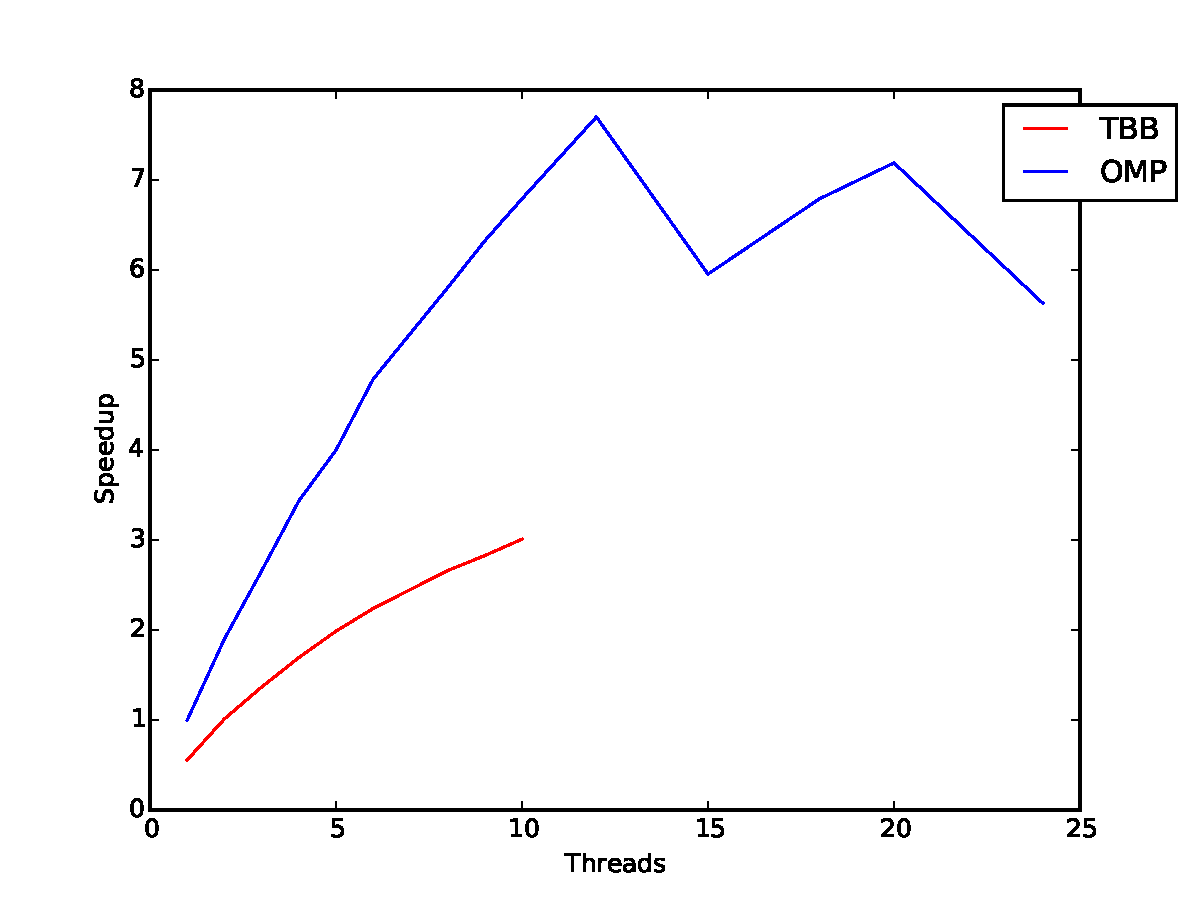
\includegraphics[width=0.5\tw]{fig-results-tbb-omp.pdf}

  \caption{\textbf{Strong scaling of OMP and TBB without vectorization --} Strong scaling results for a minibatch size of 360 for OMP and TBB without vectorization. The original author's code (TBB) does not work for more than 10 threads and thus results are not shown for TBB with >10 threads. Note the dip when OMP goes beyond 12 threads which is a result of increased communication cost across 2 chips.}

  \label{fig-results-tbb-omp}

  \centering
  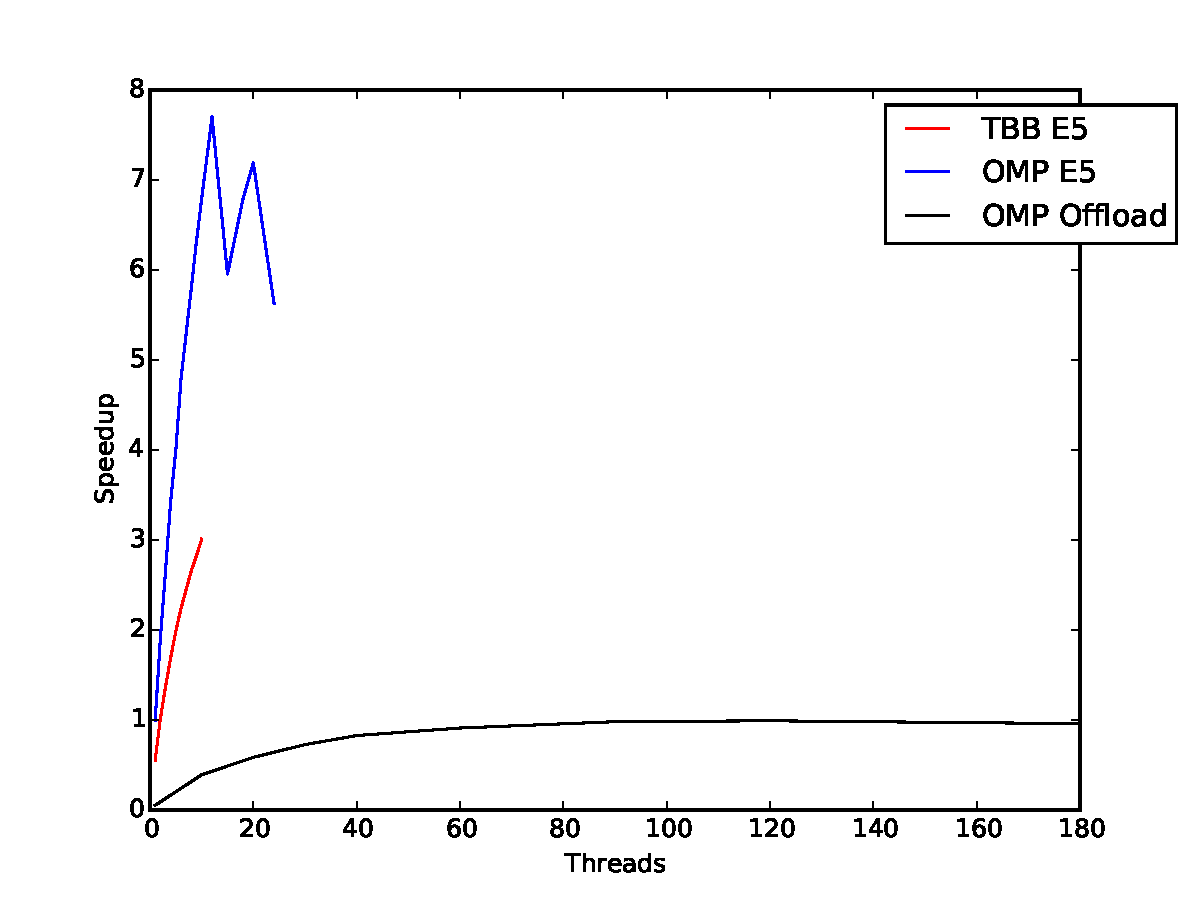
\includegraphics[width=0.5\tw]{fig-results-mic.pdf}

  \caption{\textbf{Strong scaling of offloaded MIC without vectorization --} Strong scaling results for offloaded MIC code as compared to TBB and OMP on the compute node. The offloaded MIC code performs poorly, likely due to too much serial work or lack of vectorization.}

  \label{fig-results-mic}

\end{figure}
